\documentclass[12pt]{article}
\usepackage[legalpaper, portrait, margin=1.25in]{geometry}
\usepackage{amsthm}
\usepackage{amsmath}
\usepackage{amsfonts}
\usepackage{amssymb}
\usepackage{amsrefs}
\usepackage[utf8]{inputenc}
\usepackage{titling}
\usepackage{scrextend}
\usepackage{url}
\usepackage{microtype}
\usepackage{svg}
\usepackage{shellesc}

\newenvironment{Figure}
  {\par\medskip\noindent\minipage{\linewidth}}
  {\endminipage\par\medskip}

\usepackage{multicol, caption}

\title{Piecewise Polynomials \\
    {\large Real Analysis II Investigation Assignment}}
\author{Lucas LaValva}
\date{\today}


\usepackage{fancyhdr}
\pagestyle{fancy}
\lhead{\theauthor}
\rhead{Investigation Assignment}

\begin{document}
\maketitle

\begin{abstract}
    This is a paper about polynomial interpolation.
\end{abstract}

\begin{multicols*}{2}
    \section{Introduction}

    The rapid improvements in computation throughout the past fifty years have opened many doors for mathematicians, and given them the opportunity to approach problems from a radically different angle. In addition, this new perspective has enflamed many classes of problems that had not previously been explored heavily. Two topics that frequently pertain to computational mathematics are compression of data and, more obviously, efficiency of computation. The compression of complicated mathematical constructs into smaller amounts of information is more often than not an exploration of the tradeoff between ``amount of information'' and the accuracy of what it represents.

    With current algorithms and technology, triginometric functions are computationally expensive to calculate. As such, many programs that require large volumes of triginometry keep a table of approximate values and refer to it instead of doing computations on the fly. As demand for precision increases, the size of this table must also increase rapidly. Therefore, other options have been considered for fast calculation of sine. One such method is polynomial interpolation. (Of course, the sine curve is a very simple example so methods like using the first few terms of its Taylor series are often more effective)

    % TODO: Add more to the introduction

    \section{Polynomial \\
      Interpolation}

    Polynomial interpolation \cite{enwiki:polynomial_interpolation} is a method for generating an infinitely differentiable function that passes through a one-to-one set of points in $\mathbb{R}_2$. In the examples below, evenly spaced points are placed on a sine curve and polynomials are constructed to pass through each of those points (depicted in orange).

    \begin{Figure}
        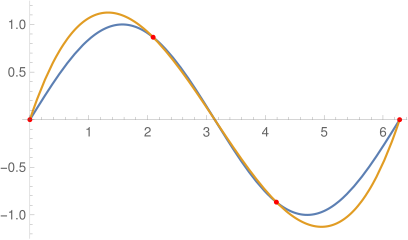
\includegraphics[width=\linewidth]{Images/SineInterpolation_EvenlySpaced/sin_interpolation_4.png}
        \captionof{figure}{4 evenly spaced points (sin)}
    \end{Figure}
    \begin{Figure}
        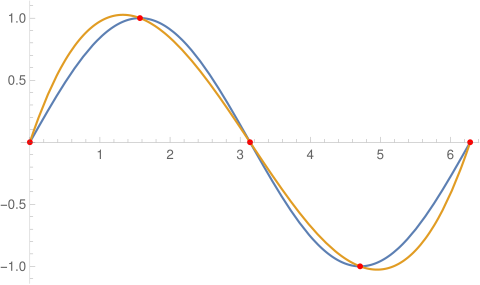
\includegraphics[width=\linewidth]{Images/SineInterpolation_EvenlySpaced/sin_interpolation_5.png}
        \captionof{figure}{5 evenly spaced points (sin)}
    \end{Figure}
    \begin{Figure}
        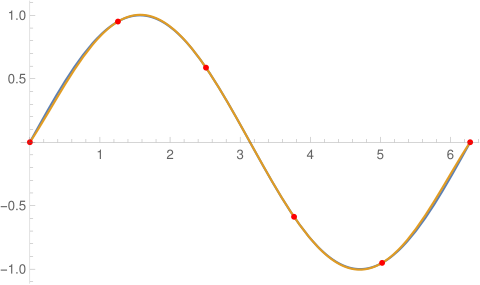
\includegraphics[width=\linewidth]{Images/SineInterpolation_EvenlySpaced/sin_interpolation_6.png}
        \captionof{figure}{6 evenly spaced points (sin)}
    \end{Figure}

    These polynomials are calculated using a method called \textbf{Lagrange Interpolation} \cite{enwiki:lagrange_polynomial}\cite{mathworld:lagrange_polynomial}. To preform this method, we begin with $n$ data points that will be referred to as $(x_1, y_1), (x_2, y_2), \ldots, (x_n, y_n)$. In order to find a polynomial that passes through all of these points, we use
    \begin{align*}
        P(x) & = \sum_{j=1}^n\left(y_j\prod_{\substack{k=1 \\ k\neq j}}^n
        \frac{x-x_k}{x_j-x_k} \right)
    \end{align*}
    or, written more explicitly,
    \begin{align*}
         & \phantom{+} y_1\frac{(x-x_2)(x-x_3)\ldots(x-x_n)}{(x_1-x_2)(x_1-x_3)\ldots(x_1-x_n)} \\
         & + y_2\frac{(x-x_1)(x-x_3)\ldots(x-x_n)}{(x_2-x_1)(x_2-x_3)\ldots(x_2-x_n)}           \\
         & \vdots                                                                               \\
         & + y_n\frac{(x-x_1)(x-x_2)\ldots(x-x_{n-1})}{(x_n-x_1)(x_n-x_2)\ldots(x_n-x_{n-1})}.
    \end{align*}
    In most cases, this formula works very well. In fact, as the number of points tends towards infinity, 


    \bibliographystyle{acm}
    \bibliography{investigationAssignment}
\end{multicols*}

\end{document}